\section{Overview}


This tutorial demonstrates how to set up and perform an analysis for different substitution models. 
The substitution models used in molecular evolution are continuous time Markov models, which are fully characterized by their instantaneous-rate matrix:
\begin{equation*}
Q = \begin{pmatrix} -\mu_A & \mu_{GA} & \mu_{CA} & \mu_{TA} \\
\mu_{AG} & -\mu_G  & \mu_{CG} & \mu_{TG} \\
\mu_{AC} & \mu_{GC} & -\mu_C  & \mu_{TC} \\
\mu_{AT} & \mu_{GT} & \mu_{CT} & -\mu_T 
\end{pmatrix} \mbox{  ,}
\end{equation*}
where $\mu_{ij}$ represents the instantaneous rate of substitution from state $i$ to state $j$. Given the instantaneous-rate matrix, $Q$, we can compute the corresponding transition probabilities for a branch of length $t$, $P(t)$, by exponentiating the rate matrix:
\begin{equation*}
P(t) = \begin{pmatrix}          
p_{AA}(t) & p_{GA}(t) & p_{CA}(t) & p_{TA}(t) \\
p_{AG}(t) & p_{GG}(t) & p_{CG}(t) & p_{TG}(t) \\
p_{AC}(t) & p_{GC}(t) & p_{CC}(t) & p_{TC}(t) \\
p_{AT}(t) & p_{GT}(t) & p_{CT}(t) & p_{TT}(t)
\end{pmatrix} = e^{Qt} = \sum_{j=0}^\infty\frac{tQ^j}{j!} \mbox{  .}
\end{equation*}
Each specific substitution model has a uniquely defined rate matrix, $Q$.


In this tutorial you will create a phylogenetic model for the evolution of DNA sequences under common models, including JC, HKY85, GTR, GTR+Gamma and GTR+Gamma+I substitution models.
For all of these models you will perform an MCMC analysis to estimate phylogeny and other model parameters.

\subsection*{Requirements}
We assume that you have read and hopefully completed the following tutorials:
\begin{itemize}
\item RB\_Getting\_Started
\item RB\_Basics\_Tutorial
\end{itemize}



%
%\subsection*{Analysis Functions}
%
\newpage
\FloatBarrier
\section{Example: Character Evolution under the Jukes-Cantor Substitution Model}

\bigskip
\subsection{Getting Started}

The first section of this exercise involves:
(1) setting up a Jukes-Cantor (JC) substitution model for an alignment of the cytochrome b subunit;
(2) approximating the posterior probability of the tree topology and branch lengths (and all other parameters) using MCMC, and; 
(3) summarizing the MCMC output by computing the maximum \textit{a posteriori} tree. 


The general structure of the model is represented in Figure~\ref{fig:jc}.
\begin{figure}[h!]
\centering
\fbox{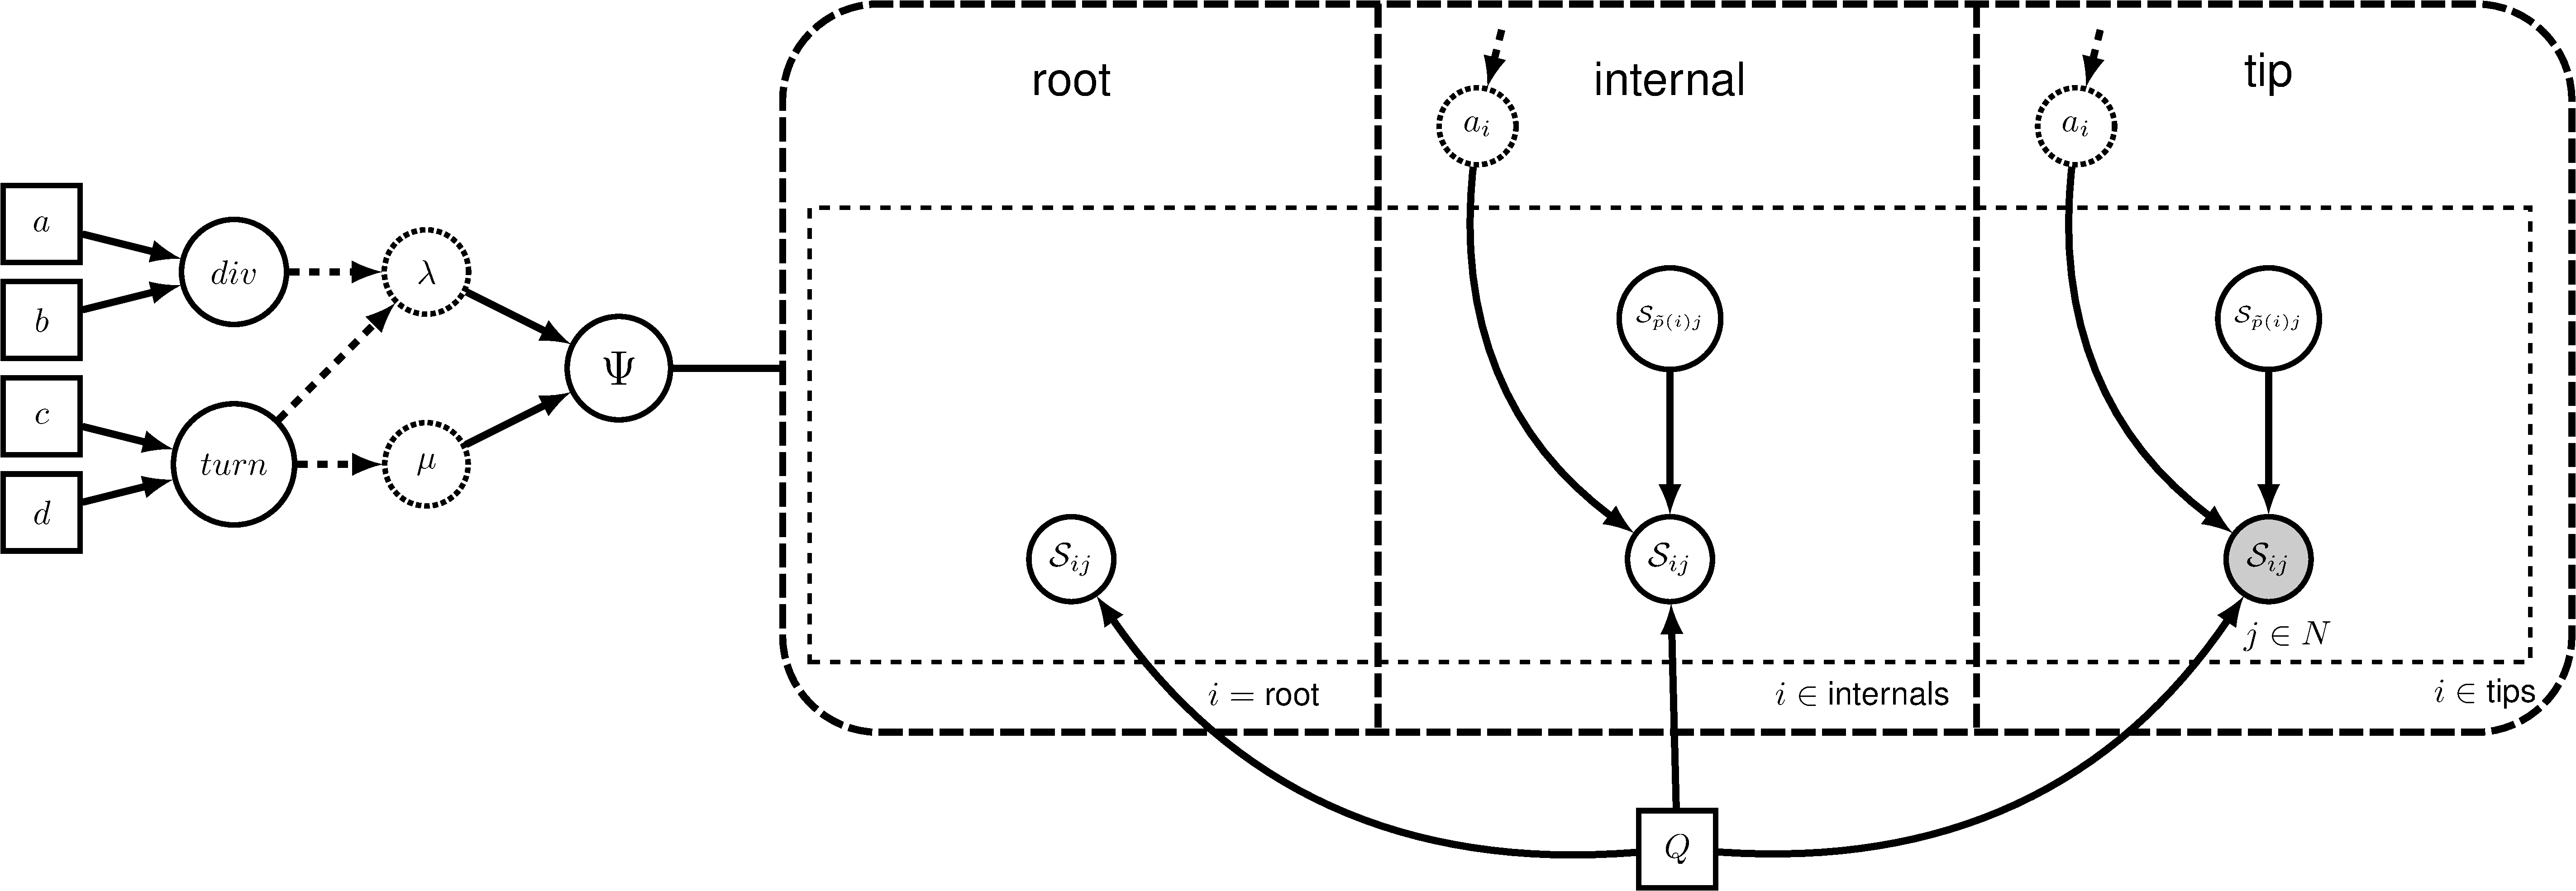
\includegraphics[width=\textwidth,angle=0]{\ResourcePath figures/jc_graphical_model.pdf}}
\caption{\small Graphical model representation of a simple phylogenetic model. 
The graphical model shows the dependencies between the parameters.
Here, the rate matrix $Q$ is constant variable because it is fixed and does not depend on any parameters.
The only free parameters of this model, the unconstrained Jukes-Cantor model, are the tree topology $\Psi$ and the branch lengths $\nu_i$.
}
\label{fig:jc}
\end{figure}
We first consider the simplest substitution model, the Jukes-Cantor \citep{Jukes1969} substitution model.
The rate matrix is defined as
\begin{equation*}
Q_{JC69} = \begin{pmatrix} 
{*} & {1} & {1} & {1} \\ 
{1} & {*} & {1} & {1} \\ 
{1} & {1} & {*} & {1} \\ 
{1} & {1} & {1} & {*}  
\end{pmatrix} \mbox{  ,}
\end{equation*}
which has the advantage that the transition probability matrix can be computed analytically:
\begin{equation*}
P_{JC69} = \begin{pmatrix} {{1\over4} + {3\over4}e^{-t\mu}} & {{1\over4} - {1\over4}e^{-t\mu}} & {{1\over4} - {1\over4}e^{-t\mu}} & {{1\over4} - {1\over4}e^{-t\mu}} \\\\ {{1\over4} - {1\over4}e^{-t\mu}} & {{1\over4} + {3\over4}e^{-t\mu}} & {{1\over4} - {1\over4}e^{-t\mu}} & {{1\over4} - {1\over4}e^{-t\mu}} \\\\ {{1\over4} - {1\over4}e^{-t\mu}} & {{1\over4} - {1\over4}e^{-t\mu}} & {{1\over4} + {3\over4}e^{-t\mu}} & {{1\over4} - {1\over4}e^{-t\mu}} \\\\ {{1\over4} - {1\over4}e^{-t\mu}} & {{1\over4} - {1\over4}e^{-t\mu}} & {{1\over4} - {1\over4}e^{-t\mu}} & {{1\over4} + {3\over4}e^{-t\mu}}  
\end{pmatrix} \mbox{  .}
\end{equation*}
In the later exercises you will be asked to specify more complex substitution models.
\textbf{Don't be scared by the math!}
\RevBayes~will take care of all the computations for you.
Here we only provide some of the equations for the models in case you might be interested in the details.
You will be able to complete the exercises without understanding the underlying math.


The files for this example analysis are provided for you, which can easily be run using the \cl{source()} function in the \RevBayes~console:
{\tt \begin{snugshade*}
\begin{lstlisting}
source("RevBayes_scripts/JukesCantor.Rev")
\end{lstlisting}
\end{snugshade*}}

If everything loaded properly, then you should see the program initiate the Markov chain Monte Carlo analysis that estimates the posterior distribution. 
If you continue to let this run, then you will see it output the states of the Markov chain once the MCMC analysis begins. 
(It is worth noting, however, that the file \cl{JukesCantor.Rev} performs shorter runs with fewer generations for the purposes of illustration.)

Ultimately, this is how you will execute most analyses in \RevBayes~and the full specification of the model and analyses are contained in the sourced files. 
You could easily run this entire analysis on your own data by substituting your data file name for that in the model-specification file. 
However, it is important to understand the components of the model to be able to take full advantage of the flexibility and richness of \RevBayes.
Furthermore, without inspecting the \Rev~scripts sourced in \cl{JukesCantor.Rev}, you may end up inadvertently performing inappropriate analyses on your dataset, which would be a waste of your time and CPU cycles. 
The next steps will walk you through the full specification of the model and MCMC analyses. 

\bigskip

\subsection{Loading the Data}

\noindent \\ \impmark Download data and output files (if you don't have them already) from: \href{http://revbayes.github.io/tutorials.html}{http://revbayes.github.io/tutorials.html}


First load in the sequences using the \cl{readDiscreteCharacterData()} function. 
%This function returns a \textit{vector} of data matrices and, even though there is only one element in the vector, we must index that element using the \cl{[1]} notation. 
%(You will also note that list indexing in Rev starts with \cl{1} like in the R language.)
{\tt \begin{snugshade*}
\begin{lstlisting}
data <- readDiscreteCharacterData("data/primates_cytb.nex")
\end{lstlisting}
\end{snugshade*}}
Executing these lines initializes the data matrix as the respective \Rev~variables. 
To report the current value of any variable, simply type the variable name and press enter. For the \cl{data} matrix, this provides information about the alignment:
{\tt \begin{snugshade*}
\begin{lstlisting}
data
|*   DNA character matrix with 24 taxa and 1141 characters
|*   =====================================================
|*   Origination:                      primates_cytb.nex
|*   Number of taxa:                   24
|*   Number of included taxa:          24
|*   Number of characters:             1141
|*   Number of included characters: 1141
|*   Datatype:                         DNA
\end{lstlisting}
\end{snugshade*}}


Next we will specify some useful variables based on our dataset. The variable \cl{data} has \textit{member functions} that we can use to retrieve information about the dataset. 
These include the number of species (\cl{n\_species}), the tip labels (\cl{names}), and the number of internal branches (\cl{n\_branches}).
Each of these variables will be necessary for setting up different parts of our model.
{\tt \begin{snugshade*}
\begin{lstlisting}
n_species <- data.ntaxa()
names <- data.names()	
n_branches <- 2 * n_species - 3 
\end{lstlisting}
\end{snugshade*}}

Additionally, we set up a counter variable for the number of moves that we already added to our analysis.
[Recall that moves are algorithms used to propose new parameter values during the MCMC simulation.]
This will make it much easier if we extend the model or analysis to include additional moves or to remove some moves.
{\tt \begin{snugshade*}
\begin{lstlisting}
mi = 0 
\end{lstlisting}
\end{snugshade*}}
You may have noticed that we used the \cl{=} operator to create the move-index.
This simply means that the variable is not part of the model.
You will later see that we use this operator more often, \EG when we create moves and monitors.

With the data loaded, we can now proceed to specify our Jukes-Cantor model.

\subsection{Jukes-Cantor Substitution Model}

A given substitution model is defined by its corresponding instantaneous-rate matrix, $Q$.
The Jukes-Cantor substitution model does not have any free parameters (as the substitution rates are all assumed to be equal), so we can define it as a constant variable.
The function \cl{fnJC(n)} will create an instantaneous-rate matrix for character with $n$ states.
Since we use DNA data here, we create a 4x4 instantaneous-rate matrix:
{\tt \begin{snugshade*}
\begin{lstlisting}
Q <- fnJC(4) 
\end{lstlisting}
\end{snugshade*}}
You can see the rates of the $Q$ matrix by typing
{\tt \begin{snugshade*}
\begin{lstlisting}
Q
|*   [ [ -1.0000, 0.3333, 0.3333, 0.3333 ] ,
|*     0.3333, -1.0000, 0.3333, 0.3333 ] ,
|*     0.3333, 0.3333, -1.0000, 0.3333 ] ,
|*     0.3333, 0.3333, 0.3333, -1.0000 ] ]
\end{lstlisting}
\end{snugshade*}}
As you can see, all substitution rates are equal.


\subsection{Tree Topology and Branch Lengths}

The tree topology and branch lengths are stochastic nodes in our model. 
In Figure \ref{fig:jc}, the tree topology is denoted $\Psi$ and the length of the branch leading to node $i$ is $\nu_i$.

We will assume that all possible labeled, unrooted tree topologies have equal probability. This is the \cl{dnUniformTopology()} distribution in \RevBayes. Specify the \cl{topology} stochastic node by passing in the tip labels \cl{names} to the \cl{dnUniformTopology()} distribution:
{\tt \begin{snugshade*}
\begin{lstlisting}
topology ~ dnUniformTopology(names)
\end{lstlisting}
\end{snugshade*}}

Some types of stochastic nodes can be updated by a number of alternative moves. 
Different moves may explore parameter space in different ways, and it is possible to use multiple different moves for a given parameter to improve mixing. 
In the case of our unrooted tree topology, for example, we can use both a nearest-neighbor interchange move (\cl{mvNNI}) and a subtree-prune and regrafting move (\cl{mvSPR}). 
These moves do not have tuning parameters associated with them, thus you only need to pass in the \cl{topology} node and \cl{weight} 
{\tt \begin{snugshade*}
\begin{lstlisting}
moves[++mi] = mvNNI(topology, weight=1.0)
moves[++mi] = mvSPR(topology, weight=1.0)
\end{lstlisting}
\end{snugshade*}}
The weight specifies how often the move will be applied either on average per iteration or relative to all other moves.
Have a look at the MCMC tutorial for more details about moves and MCMC strategies: \href{http://revbayes.github.io/tutorials.html}{http://revbayes.github.io/tutorials.html}


Next we have to create a stochastic node for each of the $2N-3$ branches in our tree (where $N=$ \cl{n\_species}). 
We can do this using a \cl{for} loop --- this is a plate in our graphical model. In this loop, we can create each branch-length node and assign each move. Copy this entire block of \Rev~code into the console:
{\tt \small \begin{snugshade*}
\begin{lstlisting}
for (i in 1:n_branches) {
   br_lens[i] ~ dnExponential(10.0)
   moves[++mi] = mvScale(br_lens[i]) 
}
\end{lstlisting}
\end{snugshade*}}

It is convenient for monitoring purposes to add the tree length as deterministic variable. The tree length is simply the sum of all branch lengths.
Accordingly, the tree length can be computed using the \cl{sum()} function, which calculates the sum of any vector of values.
{\tt \begin{snugshade*}
\begin{lstlisting}
TL := sum(br_lens)
\end{lstlisting}
\end{snugshade*}}

Finally, we can create a phylogram (a phylogeny in which the branch lengths are proportional to the expected number of substitutions/site) by combining the tree topology and branch lengths.
We do this using the \cl{treeAssembly()} function, which applies the value of the $i^{th}$ member of the \cl{br\_lens} vector to the branch leading to the $i^{th}$ node in \cl{topology}. 
Thus, the \cl{phylogeny} variable is a deterministic node: 

{\tt \begin{snugshade*}
\begin{lstlisting}
phylogeny := treeAssembly(topology, br_lens)
\end{lstlisting}
\end{snugshade*}}



\subsection{Putting it All Together}

%Having specified virtually all of our phylogenetic model parameters, we can now link all of the parts in the stochastic node that will be clamped by the data. 
%The sequence substitution model is a distribution called the \textit{phylogenetic continuous-time Markov chain}, and we use the \cl{PhyloCTMC} constructor function to create this node.
% The above two sentences are a bit unclear: I think we could say something like: 
We have fully specified all of the parameters of our phylogenetic model---the tree topology with branch lengths, and the substitution model that describes how the sequence data evolved over the tree with branch lengths.  
Collectively, these parameters comprise a distribution called the \textit{phylogenetic continuous-time Markov chain}, and we use the \cl{PhyloCTMC} constructor function to create this node.
This distribution requires several input arguments: 
(1) the \cl{tree} with branch lengths; 
(2) the instantaneous-rate matrix \cl{Q}, and; 
(3) the \cl{type} of character data.
{\tt \begin{snugshade*}
\begin{lstlisting}
seq ~ dnPhyloCTMC(tree=phylogeny, Q=Q, type="DNA")
\end{lstlisting}
\end{snugshade*}}


Once the \cl{PhyloCTMC} model has been created, we can attach our sequence data to the tip nodes in the tree.
{\tt \begin{snugshade*}
\begin{lstlisting}
seq.clamp(data)
\end{lstlisting}
\end{snugshade*}}
[Note that although we assume that our sequence data are random variables---they are realizations of our phylogenetic model---for the purposes of inference, we assume that the sequence data are ``clamped''.]
When this function is called, \RevBayes~sets each of the stochastic nodes representing the tips of the tree to the corresponding sequence in the alignment. 
This essentially tells the program that we have observed data for the sequences at the tips. 

Finally, we wrap the entire model to provide convenient access to the DAG. 
To do this, we only need to give the \cl{model()} function a single node. 
With this node, the \cl{model()} function can find all of the other nodes by following the arrows in the graphical model:
{\tt \begin{snugshade*}
\begin{lstlisting}
mymodel = model(Q)
\end{lstlisting}
\end{snugshade*}}

Now we have specified a simple molecular phylogenetic analysis---each parameter of the model will be estimated from every site in our alignment.
If we inspect the contents of \cl{mymodel} we can review all of the nodes in the DAG:
{\tt \begin{snugshade*}
\begin{lstlisting}
mymodel
\end{lstlisting}
\end{snugshade*}}

\bigskip
\subsection{Performing an MCMC Analysis Under the Uniform Model}

In this section, will describe how to set up the MCMC sampler and summarize the resulting posterior distribution of trees. 

\subsubsection{Specifying Monitors}

For our MCMC analysis, we need to set up a vector of \textit{monitors} to record the states of our Markov chain. 
The monitor functions are all called \cl{mn*}, where \cl{*} is the wildcard representing the monitor type.
First, we will initialize the model monitor using the \cl{mnModel} function. This creates a new monitor variable that will output the states for all model parameters when passed into a MCMC function. 
{\tt \begin{snugshade*}
\begin{lstlisting}
monitors[1] = mnModel(filename="output/primates_cytb_JC_posterior.log",printgen=10, separator = TAB)
\end{lstlisting}
\end{snugshade*}}

The \cl{mnFile} monitor will record the states for only the parameters passed in as arguments. We use this monitor to specify the output for our sampled trees and branch lengths.

{\tt \begin{snugshade*}
\begin{lstlisting}
monitors[2] = mnFile(filename="output/primates_cytb_JC_posterior.trees",printgen=10, separator = TAB, phylogeny)
\end{lstlisting}
\end{snugshade*}}


Finally, create a screen monitor that will report the states of specified variables to the screen with \cl{mnScreen}:
{\tt \begin{snugshade*}
\begin{lstlisting}
monitors[3] = mnScreen(printgen=1000, TL)
\end{lstlisting}
\end{snugshade*}}

\subsubsection{Initializing and Running the MCMC Simulation}

With a fully specified model, a set of monitors, and a set of moves, we can now set up the MCMC algorithm that will sample parameter values in proportion to their posterior probability. The \cl{mcmc()} function will create our MCMC object:
{\tt \begin{snugshade*}
\begin{lstlisting}
mymcmc = mcmc(mymodel, monitors, moves)
\end{lstlisting}
\end{snugshade*}}


We may wish to run the \cl{.burnin()} member function.
% if we wish to pre-run the chain and discard the initial states. 
% I think you might want to add a brief explanation here, something like:
Recall that this function \textbf{does not} specify the number of states that we wish to discard from the MCMC analysis as burnin (i.e., the samples collected before the chain converges to the stationary distribution).  
Instead, the \cl{.burnin()} function specifies a \textit{completely separate} preliminary MCMC analysis that is used to tune the scale of the moves to improve mixing of the MCMC analysis.
{\tt \begin{snugshade*}
\begin{lstlisting}
mymcmc.burnin(generations=10000,tuningInterval=1000)
\end{lstlisting}
\end{snugshade*}}


Now, run the MCMC:
{\tt \begin{snugshade*}
\begin{lstlisting}
mymcmc.run(generations=30000)
\end{lstlisting}
\end{snugshade*}}

When the analysis is complete, you will have the monitored files in your output directory.


Methods for visualizing the marginal densities of parameter values are not currently available in \RevBayes~itself. 
Thus, it is important to use programs like \texttt{Tracer} \citep{Rambaut2011} to evaluate mixing and non-convergence. (\RevBayes~does, however, have a tool for convergence assessment called \cl{beca}.)

\noindent \\ \impmark Look at the file called \cl{output/primates\_cytb\_JC\_posterior.log} in \texttt{Tracer}.


\subsection{Exercise 1}

We are interested in the phylogenetic relationship of the Tarsiers. Therefore, we need to summarize the trees sampled from the posterior distribution.
\RevBayes~can summarize the sampled trees by reading in the tree-trace file:
{\tt \begin{snugshade*}
\begin{lstlisting}
treetrace = readTreeTrace("output/primates_cytb_JC_posterior.trees", treetype="non-clock")
treetrace.summarize()
\end{lstlisting}
\end{snugshade*}}
The \cl{mapTree()} function will summarize the tree samples and write the maximum \textit{a posteriori} tree to file:
{\tt \begin{snugshade*}
\begin{lstlisting}
mapTree(treetrace,"output/primates_cytb_JC.tree")
\end{lstlisting}
\end{snugshade*}}
Fill in the following table as you go through the tutorial.

\begin{Form}
\begin{table}[h!]
\centering
\caption{\small Posterior probabilities of phylogenetic relationship$^*$.}
\resizebox{\textwidth}{!}{%
\begin{tabular}{l c c c c c}
\hline
\textbf{Model} & \textit{Lemuroidea} & \textit{Lorisoidea} & \textit{Platyrrhini} & \textit{Catarrhini} & \textit{other} \\ 
\hline
\vspace{1mm}
Jukes-Cantor & \TextField[name=pp11,backgroundcolor={.85 .85 .85},color={1 0 0},height=4ex]{}  & \TextField[name=pp12,backgroundcolor={.85 .85 .85},color={0 0 1},height=4ex]{}  & \TextField[name=pp13,backgroundcolor={.85 .85 .85},color={0 0 1},height=4ex]{}  & \TextField[name=pp14,backgroundcolor={.85 .85 .85},color={0 0 1},height=4ex]{} & \TextField[name=pp15,backgroundcolor={.85 .85 .85},color={0 0 1},height=4ex]{} \\
\hline
\vspace{1mm}
HKY85 & \TextField[name=pp21,backgroundcolor={.85 .85 .85},color={1 0 0},height=4ex]{}  & \TextField[name=pp22,backgroundcolor={.85 .85 .85},color={0 0 1},height=4ex]{}  & \TextField[name=pp23,backgroundcolor={.85 .85 .85},color={0 0 1},height=4ex]{}  & \TextField[name=pp24,backgroundcolor={.85 .85 .85},color={0 0 1},height=4ex]{} & \TextField[name=pp25,backgroundcolor={.85 .85 .85},color={0 0 1},height=4ex]{} \\
\hline
\vspace{1mm}
F81 & \TextField[name=pp31,backgroundcolor={.85 .85 .85},color={1 0 0},height=4ex]{}  & \TextField[name=pp32,backgroundcolor={.85 .85 .85},color={0 0 1},height=4ex]{}  & \TextField[name=pp33,backgroundcolor={.85 .85 .85},color={0 0 1},height=4ex]{}  & \TextField[name=pp34,backgroundcolor={.85 .85 .85},color={0 0 1},height=4ex]{} & \TextField[name=pp35,backgroundcolor={.85 .85 .85},color={0 0 1},height=4ex]{} \\
\hline
\vspace{1mm}
GTR & \TextField[name=pp41,backgroundcolor={.85 .85 .85},color={1 0 0},height=4ex]{}  & \TextField[name=pp42,backgroundcolor={.85 .85 .85},color={0 0 1},height=4ex]{}  & \TextField[name=pp43,backgroundcolor={.85 .85 .85},color={0 0 1},height=4ex]{}  & \TextField[name=pp44,backgroundcolor={.85 .85 .85},color={0 0 1},height=4ex]{} & \TextField[name=pp45,backgroundcolor={.85 .85 .85},color={0 0 1},height=4ex]{} \\
\hline
\vspace{1mm}
GTR+$\Gamma$ & \TextField[name=pp51,backgroundcolor={.85 .85 .85},color={1 0 0},height=4ex]{}  & \TextField[name=pp52,backgroundcolor={.85 .85 .85},color={0 0 1},height=4ex]{}  & \TextField[name=pp53,backgroundcolor={.85 .85 .85},color={0 0 1},height=4ex]{}  & \TextField[name=pp54,backgroundcolor={.85 .85 .85},color={0 0 1},height=4ex]{} & \TextField[name=pp55,backgroundcolor={.85 .85 .85},color={0 0 1},height=4ex]{} \\
\hline
\vspace{1mm}
GTR+$\Gamma$+I & \TextField[name=pp61,backgroundcolor={.85 .85 .85},color={1 0 0},height=4ex]{}  & \TextField[name=pp62,backgroundcolor={.85 .85 .85},color={0 0 1},height=4ex]{}  & \TextField[name=pp63,backgroundcolor={.85 .85 .85},color={0 0 1},height=4ex]{}  & \TextField[name=pp64,backgroundcolor={.85 .85 .85},color={0 0 1},height=4ex]{} & \TextField[name=pp65,backgroundcolor={.85 .85 .85},color={0 0 1},height=4ex]{} \\
\hline
\vspace{1mm}
Your model 1 & \TextField[name=pp71,backgroundcolor={.85 .85 .85},color={1 0 0},height=4ex]{}  & \TextField[name=pp72,backgroundcolor={.85 .85 .85},color={0 0 1},height=4ex]{}  & \TextField[name=pp73,backgroundcolor={.85 .85 .85},color={0 0 1},height=4ex]{}  & \TextField[name=pp74,backgroundcolor={.85 .85 .85},color={0 0 1},height=4ex]{} & \TextField[name=pp75,backgroundcolor={.85 .85 .85},color={0 0 1},height=4ex]{} \\
\hline
\vspace{1mm}
Your model 2 & \TextField[name=pp81,backgroundcolor={.85 .85 .85},color={1 0 0},height=4ex]{}  & \TextField[name=pp82,backgroundcolor={.85 .85 .85},color={0 0 1},height=4ex]{}  & \TextField[name=pp83,backgroundcolor={.85 .85 .85},color={0 0 1},height=4ex]{}  & \TextField[name=pp84,backgroundcolor={.85 .85 .85},color={0 0 1},height=4ex]{} & \TextField[name=pp85,backgroundcolor={.85 .85 .85},color={0 0 1},height=4ex]{} \\
\hline
\vspace{1mm}
Your model 3 & \TextField[name=pp91,backgroundcolor={.85 .85 .85},color={1 0 0},height=4ex]{}  & \TextField[name=pp92,backgroundcolor={.85 .85 .85},color={0 0 1},height=4ex]{}  & \TextField[name=pp93,backgroundcolor={.85 .85 .85},color={0 0 1},height=4ex]{}  & \TextField[name=pp94,backgroundcolor={.85 .85 .85},color={0 0 1},height=4ex]{} & \TextField[name=pp95,backgroundcolor={.85 .85 .85},color={0 0 1},height=4ex]{} \\
\hline
{\footnotesize{$^*$you can edit this table}}\\
\end{tabular}}
\label{tab:pp}
\end{table}
\end{Form}




\newpage
\section{The Hasegawa-Kishino-Yano (HKY) 1985 Substitution Model}

The Jukes-Cantor model assumes that all substitution rates are equal, which also implies that also the stationary frequencies of the four bases are equal.
These assumptions are not very biologically reasonable, so we might wish to consider a more realistic substitution model that relaxes some of these assumptions.
For example, we might allow stationary frequencies, $\pi$, to be unequal, and allow rates of transition and transversion substitutions to differ, $\kappa$.
This corresponds to the substitution model proposed by \citet[][HKY]{Hasegawa1985}, which is specified with the following instantaneous-rate matrix: 
\begin{equation*}
Q_{HKY} = \begin{pmatrix} 
{*} & {\kappa\pi_C} & {\pi_G} & {\pi_T} \\ 
{\kappa\pi_A} & {*} & {\pi_C} & {\pi_T} \\ 
{\pi_A} & {\pi_C} & {*} & {\kappa\pi_T} \\ 
{\pi_A} & {\pi_C} & {\kappa\pi_G} & {*}  
\end{pmatrix} \mbox{  .}
\end{equation*}

\noindent \\ \impmark Use the file \cl{JukesCantor.Rev} as a starting point for the HKY analysis.

Note that we are adding two new variables to our model.
We can define a variable \cl{pi} for the stationary frequencies that are drawn from a flat Dirichlet distribution by
{\tt \begin{snugshade*}
\begin{lstlisting}
pi_prior <- v(1,1,1,1) 
pi ~ dnDirichlet(pi_prior)
\end{lstlisting}
\end{snugshade*}}
Since \cl{pi} is a stochastic variable, we need to specify a move to propose updates to it.
A good move on variables drawn from a Dirichlet distribution is the \cl{mvSimplexElementScale}.
This move randomly takes an element from the simplex, proposes a new value for it drawn from a Beta distribution, and then rescales all values of the simplex to sum to 1 again.
{\tt \begin{snugshade*}
\begin{lstlisting}
moves[++mi] = mvSimplexElementScale(pi, weight=4.0)
\end{lstlisting}
\end{snugshade*}}

The second new variable is $\kappa$, which specifies the ratio of transition-transversion rates.
$\kappa$ needs to be a positive-real number and a natural choice as the prior distribution is the lognormal distribution:
{\tt \begin{snugshade*}
\begin{lstlisting}
kappa ~ dnLnorm(0.0,1.25)
\end{lstlisting}
\end{snugshade*}}
Again, we need to specify a move for this new stochastic variable.
A simple scaling move should do the job.
{\tt \begin{snugshade*}
\begin{lstlisting}
moves[++mi] = mvScale(kappa, weight=1.0)
\end{lstlisting}
\end{snugshade*}}

Finally, we need to create the HKY instantaneous-rate matrix using the \cl{fnHKY} function:
{\tt \begin{snugshade*}
\begin{lstlisting}
Q := fnHKY(kappa,pi)
\end{lstlisting}
\end{snugshade*}}
This should be all for the HKY model.

\noindent \\ \impmark Don't forget to change the output file names, otherwise your old analyses files will be overwritten.

\subsection{Exercise 2}

\begin{itemize}
\item Copy the file called  \cl{JukesCantor.Rev} and modify it by including the new parameters so that you specify the HKY substitution model for analysis.
\item Run an MCMC analysis to estimate the posterior distribution.
\item Are the resulting estimates of the base frequencies equal? 
	If not, how much do they differ? 
	Are the estimated base frequencies similar to the empirical base frequencies? 
	The empirical base frequencies are the frequencies of the characters in the alignment, which can be computed with \RevBayes~by \cl{data.empiricalBaseFrequencies()}.
\item Is the inferred rate of transition substitutions higher than the rate of transversion substitutions? If so, by how much?
\item Like the HKY model, the Felsenstein 1981 substitution model has unequal stationary frequencies, but it assumes equal transition-transversion rates \citep{Felsenstein1981}.
	Can you set up the F81 model and run an analysis?
\item Complete the table of the phylogenetic relationship of Tarsiers.
\end{itemize}






\newpage
\section{The General Time-Reversible (GTR) Substitution Model}

The HKY substitution model can accommodate unequal base frequencies and different rates of transition and transversion substitutions.
Despite these extensions, the HKY model may still be too simple in most realistic cases.
Here, we extend the HKY model to specify the General Time Reversible (GTR) substitution model \citep{Tavare1986}, which allows all six exchangeability rates to differ.
The instantaneous-rate matrix for the GTR substitution model is
\begin{equation*}
\resizebox{\textwidth}{!}{%  
$Q_{GTR} = \begin{pmatrix}
{-(x_1 + x_2 + x_3)} & {\pi_1 x_1 \over \pi_2} & {\pi_1 x_2 \over \pi_3} & {\pi_1 x_3 \over \pi_4} \\ 
{x_1} & {-({\pi_1 x_1 \over \pi_2} + x_4 + x_5)} & {\pi_2 x_4 \over \pi_3} & {\pi_2 x_5 \over \pi_4} \\ 
{x_2} & {x_4} & {-({\pi_1 x_2 \over \pi_3} + {\pi_2 x_4 \over \pi_3} + x_6)} & {\pi_3 x_6 \over \pi_4} \\  
{x_3} & {x_5} & {x_6} & {-({\pi_1 x_3 \over \pi_4} + {\pi_2 x_5 \over \pi_4} + {\pi_3 x_6 \over \pi_4})} 
\end{pmatrix} \mbox{  .} $}
\end{equation*}

\begin{figure}[h!]
\centering
\fbox{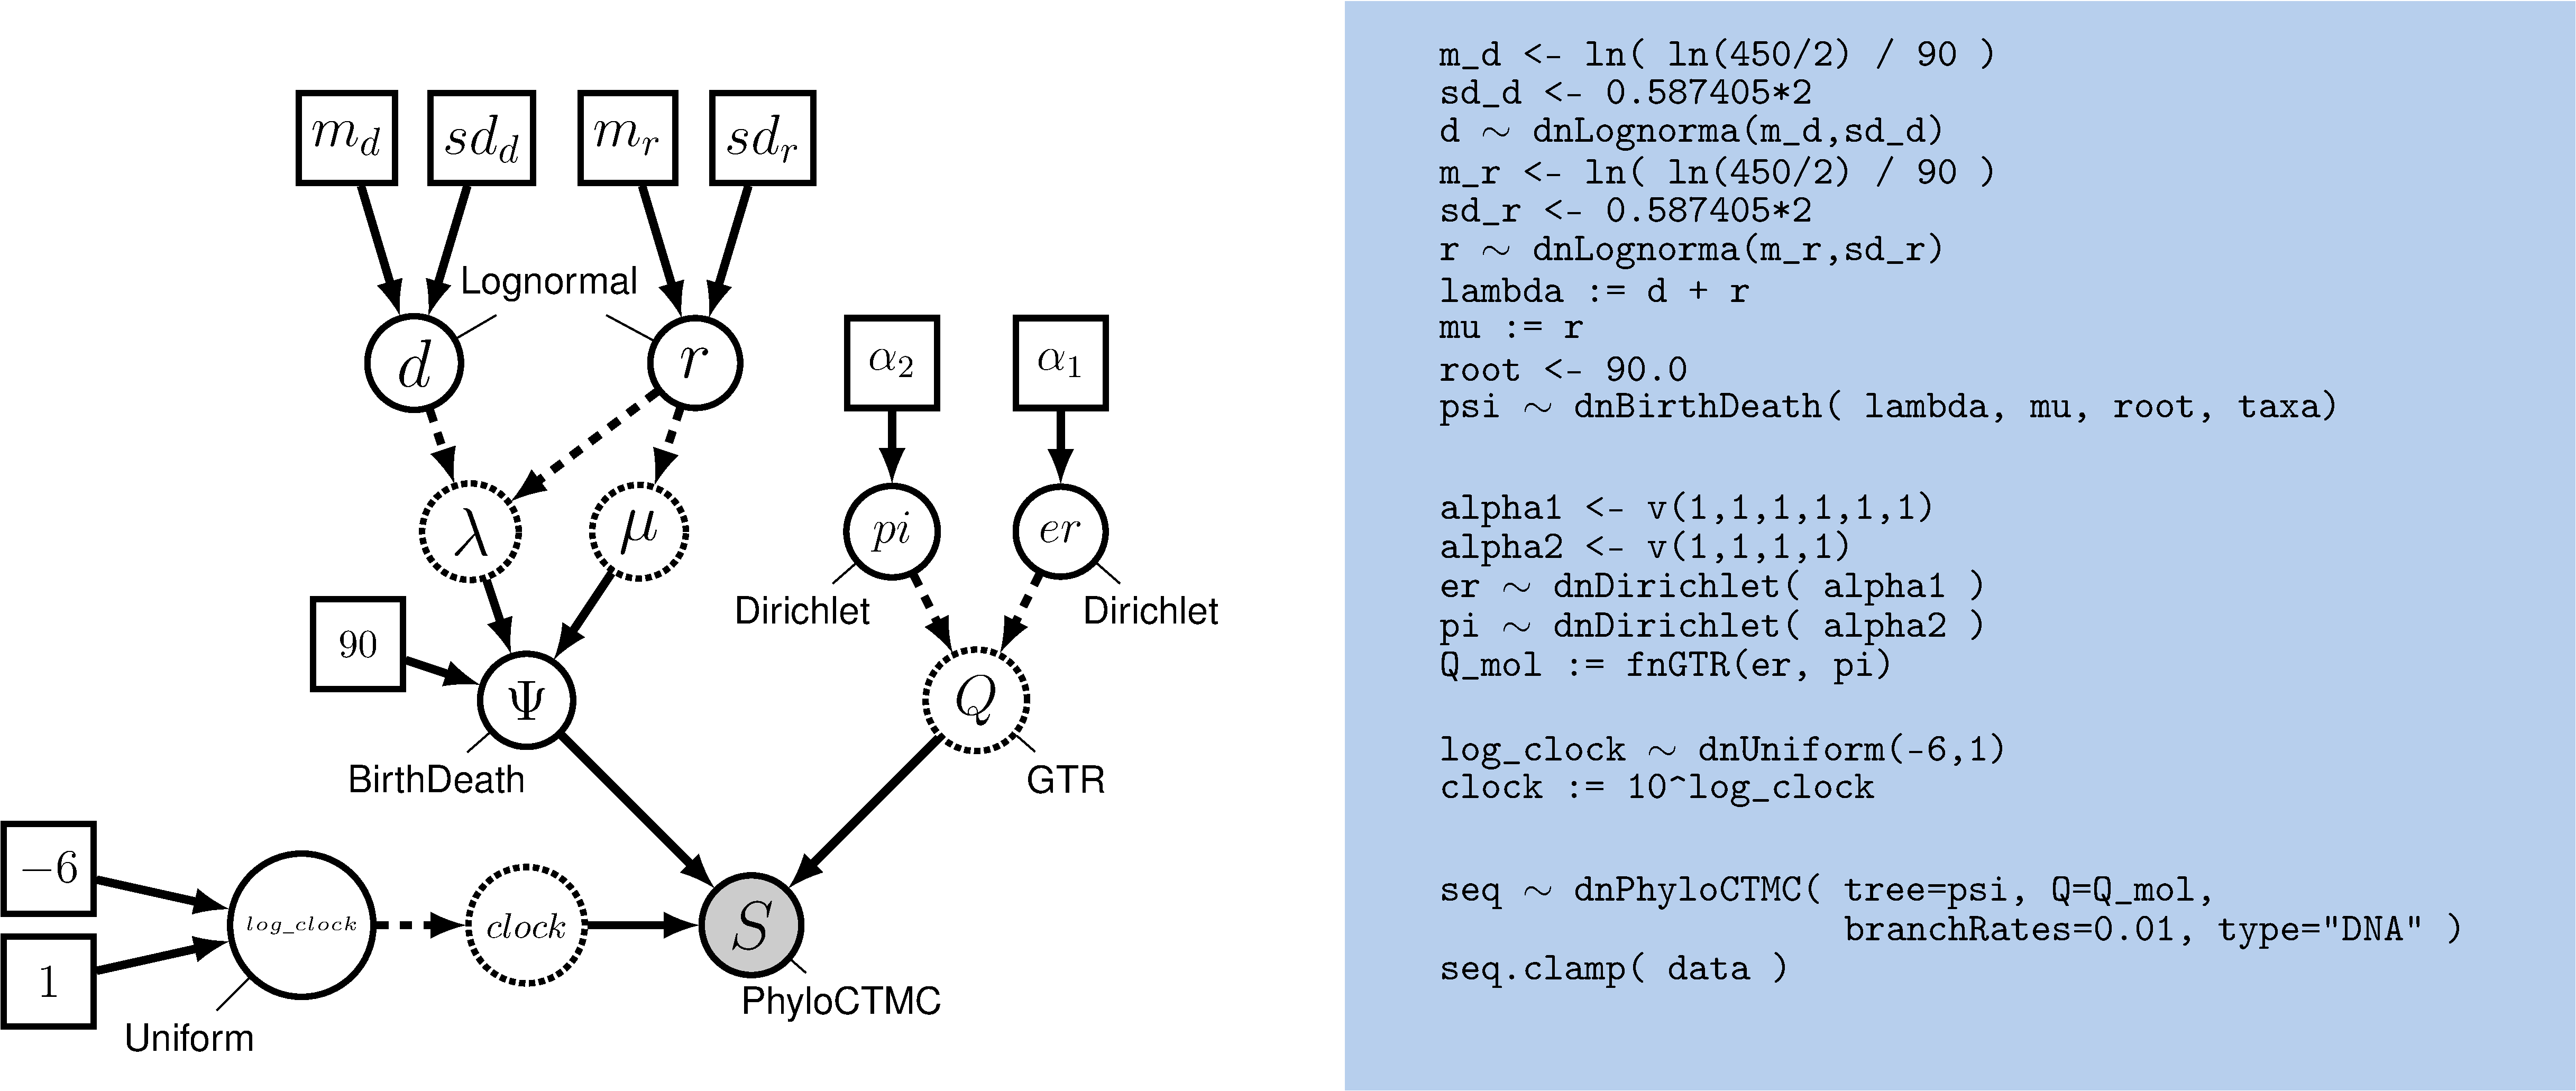
\includegraphics[width=\textwidth,angle=0]{\ResourcePath figures/gtr_graphical_model.pdf}}
\caption{\small Graphical model representation of the General Time Reversible (GTR) phylogenetic model.}
\label{fig:gtr}
\end{figure}


\subsection{Exchangeability Rate Parameters}

The GTR model requires that we define and specify a prior on the six exchangeability rates, which we will describe using a flat Dirichlet distribution.
As we did previously for the Dirichlet prior on base frequencies, we first define a constant node specifying the vector of concentration-parameter values using the \cl{v()} function:
{\tt \begin{snugshade*}
\begin{lstlisting}
er_prior <- v(1,1,1,1,1,1) 
\end{lstlisting}
\end{snugshade*}}
This node defines the concentration-parameter values of the Dirichlet prior distribution on the exchangeability rates. 
Now, we can create a stochastic node for the exchangeability rates using the \cl{dnDirichlet()} function, which takes the vector of concentration-parameter values as an argument and the \cl{\rbdn} operator. 
Together, these create a stochastic node named \cl{er} ($\theta$ in Figure \ref{fig:gtr}): 
{\tt \begin{snugshade*}
\begin{lstlisting}
er ~ dnDirichlet(er_prior)
\end{lstlisting}
\end{snugshade*}}


The Dirichlet distribution assigns probability densities to a group of parameters: e.g., those that measure proportions and must sum to 1. 
Here, we have specified a six-parameter Dirichlet prior, where each value describes one of the six relative rates of the GTR model: 
(1) $A\leftrightarrows C$; (2) $A\leftrightarrows G$; (3) $A\leftrightarrows T$; (4) $C\leftrightarrows G$; (5) $C\leftrightarrows T$; (6) $G\leftrightarrows T$. 
The input 
% why not describe these as hyperparameters?
parameters of a Dirichlet distribution are called shape (or concentration) parameters. 
The expectation and variance for each variable are related to the sum of the shape parameters.
The prior we specified above is a `flat' or symmetric Dirichlet distribution; all of the shape parameters are equal (1,1,1,1,1,1).
This describes a model that allows for equal rates of change between nucleotides, such that the expected rate for each is equal to $\frac{1}{6}$ (Figure \ref{dirichletFig}a).
%Figure \ref{dirichletFig}a shows the probability density of each rate under this model.
We might also parameterize the Dirichlet distribution such that all of the shape parameters were equal to 100, which would also specify a prior with an expectation of equal exchangeability rates (Figure \ref{dirichletFig}b). 
However, by increasing the values of the shape parameters, \cl{er\_prior <- v(100,100,100,100,100,100)}, the Dirichlet distribution will more strongly favor equal exchangeability rates; ({\it i.e.}, providing is a relatively {\em informative} prior). 
Alternatively, we might consider an asymmetric Dirichlet parameterization that could reflect a strong prior belief that transitions and transversions occurred at different rates.
For example, we might specify the prior density \cl{er\_prior <- v(4,8,4,4,8,4)}.   
Under this model, the expected rate for transversions would be $\frac{4}{32}$ and that for transitions would be $\frac{8}{32}$, and there would be greater prior probability on sets of GTR rates that matched this configuration (Figure \ref{dirichletFig}c). 
Yet another informative prior could specify that each of the six GTR rates had a different value conforming to a Dirichlet(2,4,6,8,10,12). 
This would lead to a different prior probability density for each rate parameter (Figure \ref{dirichletFig}d).
Without strong prior knowledge about the pattern of relative rates, however, we can better reflect our uncertainty by using a vague prior on the GTR rates. 
Notably, all patterns of relative rates have the same probability density under \cl{er\_prior <- v(1,1,1,1,1,1)}.
\begin{figure}[h!]
\centering
\fbox{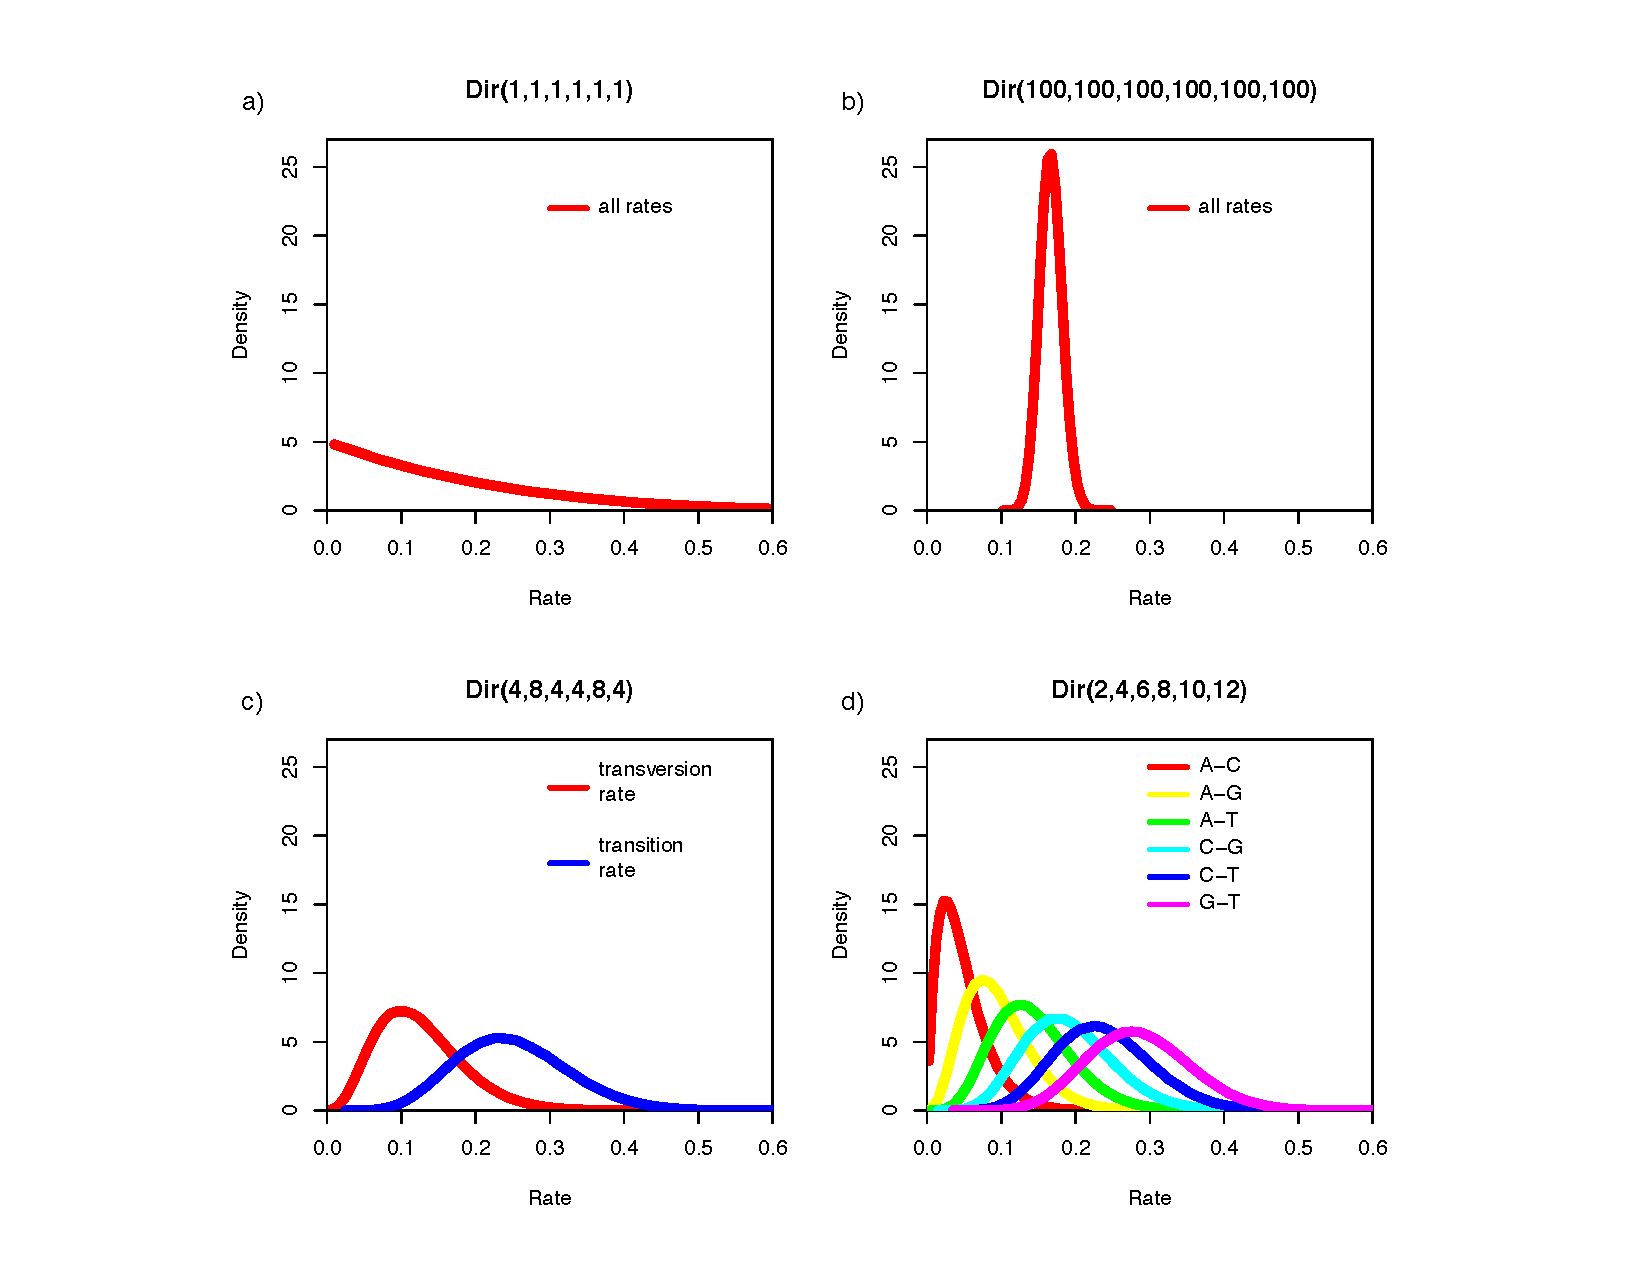
\includegraphics[width=5in]{\ResourcePath figures/dirichlet_rates.pdf}}
\caption{\small Four different examples of Dirichlet priors on exchangeability rates.}
\label{dirichletFig}
\end{figure}


For each stochastic node in our model, we must also specify a proposal mechanism if we wish to estimate that parameter. 
The Dirichlet prior on our parameter \cl{er} creates a \href{http://en.wikipedia.org/wiki/Simplex}{\textit{simplex}} of values that sum to 1. 

{\tt\small \begin{snugshade*}
\begin{lstlisting}
moves[++mi] <- mvSimplexElementScale(er, weight=3) 
\end{lstlisting}
\end{snugshade*}}

We can use the same type of distribution as a prior on the 4 stationary frequencies ($\pi_A, \pi_C, \pi_G, \pi_T$) since these parameters also represent proportions. 
Specify a flat Dirichlet prior density on the base frequencies:
{\tt \begin{snugshade*}
\begin{lstlisting}
pi_prior <- v(1,1,1,1) 
pi ~ dnDirichlet(pi_prior)
\end{lstlisting}
\end{snugshade*}}

The node \cl{pi} represents the $\pi$ node in Figure \ref{fig:gtr}.
Now add the simplex scale move on the stationary frequencies to the moves vector:
{\tt \small \begin{snugshade*}
\begin{lstlisting}
moves[++mi] <- mvSimplexElementScale(pi, weight=2)  
\end{lstlisting}
\end{snugshade*}}

We can finish setting up this part of the model by creating a deterministic node for the GTR instantaneous-rate matrix \cl{Q}. 
The \cl{fnGTR()} function takes a set of exchangeability rates and a set of base frequencies to compute the rate matrix used when calculating the likelihood of our model.
{\tt \begin{snugshade*}
\begin{lstlisting}
Q := fnGTR(er,pi)
\end{lstlisting}
\end{snugshade*}}




\subsection{Execise 3}

\begin{itemize}
\item Use one of your previous analysis file, either the \cl{JukesCantor.Rev} or \cl{HKY.Rev}, to create a GTR analysis in a new file called \cl{GTR.Rev}.
	Adapt the old analysis to be performed under the GTR substitution model. 
\item Run an MCMC analysis to estimate the posterior distribution.
\item Complete the table of the phylogenetic relationship of Tarsiers.
\end{itemize}






\newpage
\section{The Discrete Gamma Model of Among Site Rate Variation}


Members of the GTR family of substitution models assume that rates are homogeneous across sites, an assumption that is often violated by real data.
We can accommodate variation in substitution rate among sites (ASRV) by adopting the discrete-gamma model \citep{yang94a}.
This model assumes that the substitution rate at each site is a random variable that is described by a discretized gamma distribution, which has two parameters: the shape parameter, $\alpha$, and the rate parameter, $\beta$. 
In order that we can interpret the branch lengths as the expected number of substitutions per site, this model assumes that the mean site rate is equal to 1.
%Consequently, we wish to specify a gamma distribution with a mean of 1.
The mean of the gamma is equal to $\alpha/\beta$, so a mean-one gamma is specified by setting the two parameters to be equal, $\alpha=\beta$.
This means that we can fully describe the gamma distribution with the single shape parameter, $\alpha$. 
The degree of among-site substitution rate variation is inversely proportional to the value of the $\alpha$-shape parameter.
As the value of the $\alpha$-shape increases, the gamma distribution increasingly resembles a normal distribution with decreasing variance, which therefore corresponds to decreasing levels of ASRV (Figure \ref{asrhGammaFig}).
%If $\alpha = 1$, then the gamma distribution collapses to an exponential distribution with a rate parameter equal to $\beta$.
% Is it too much detail to describe the special case of |alpha = 1?
By contrast, when the value of the $\alpha$-shape parameter is $< 1$, the gamma distribution assumes a concave distribution that concentrates most of the prior density on low rates, but retains some prior mass on sites with very high rates, which therefore corresponds to high levels of ASRV (Figure \ref{asrhGammaFig}).
Note that, when $\alpha = 1$, the gamma distribution collapses to an exponential distribution with a rate parameter equal to $\beta$.


\begin{figure}[h]
\centering
\fbox{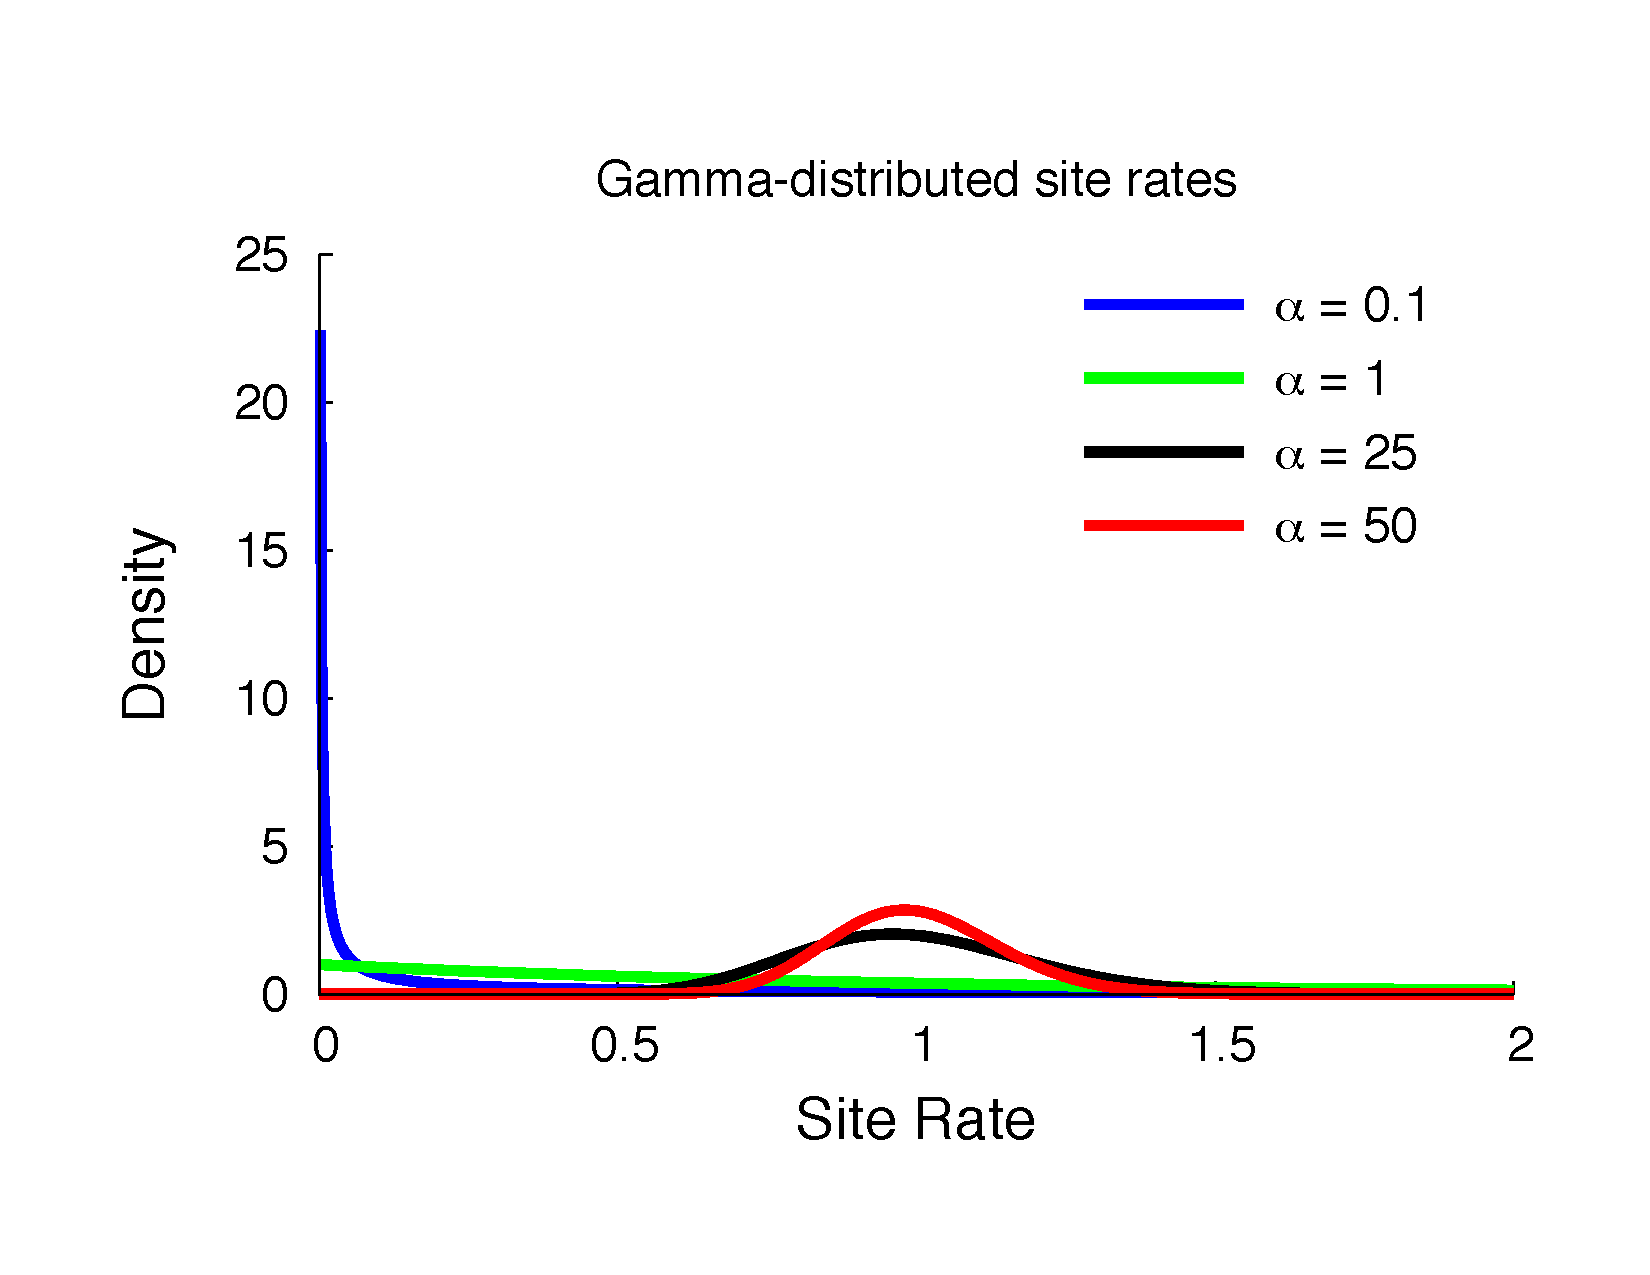
\includegraphics[width=3.5in]{\ResourcePath figures/asrh_gamma.pdf}}
\caption{\small The probability density of mean-one gamma-distributed rates for different values of the $\alpha$-shape parameter.}
\label{asrhGammaFig}
\end{figure}

We typically lack prior knowledge regarding the degree of ASRV for a given alignment.
Accordingly, rather than specifying a precise value of $\alpha$, we can instead estimate the value of the $\alpha$-shape parameter from the data.
This requires that we specify a diffuse (relatively `uninformative') prior on the $\alpha$-shape parameter.
% I think we should be careful with the our use of `uninformative' and `informative' priors---even a very vague prior can still impact the posterior, and so it is technically informative.
% This can lead to misconceptions that `flat' priors are necessarily `uninformative', which is often misleading.  So, it may be better to describe priors as more or less diffuse/informative.
For this analysis, we will use an exponential distribution with a rate parameter, \cl{shape\_prior}, equal to \cl{0.05}.
An exponential prior assigns non-zero probability on values of $\alpha$ ranging from 0 to $\infty$. 
The rate parameter of an exponential distribution, often denoted $\lambda$, controls both the mean and variance of this distribution, such that the expected (or mean) value of $\alpha$ is:
$\mathbb{E}[\alpha] = \frac{1}{\lambda}.$
Thus, if we set $\lambda=0.05$, then $\mathbb{E}[\alpha] = 20$.

This approach for accommodating ASRV is another example of a hierarchical model (Figure \ref{fig:gtrg}).
That is, variation in substitution rates across sites is addressed by applyig a site-specific rate multiplier to each of the $j$ sites, $r_j$.
These rate-multipliers are drawn from a discrete, mean-one gamma distribution; the shape of this prior distribution (and the corresponding degree of ASRV) is governed by the $\alpha$-shape parameter.
The $\alpha$-shape parameter, in turn, is treated as an exponentially distributed random variable.
Finally, the shape of the exponential prior is governed by the rate parameter, $\lambda$, which is set to a fixed value.   

\begin{figure}[h!]
\centering
\fbox{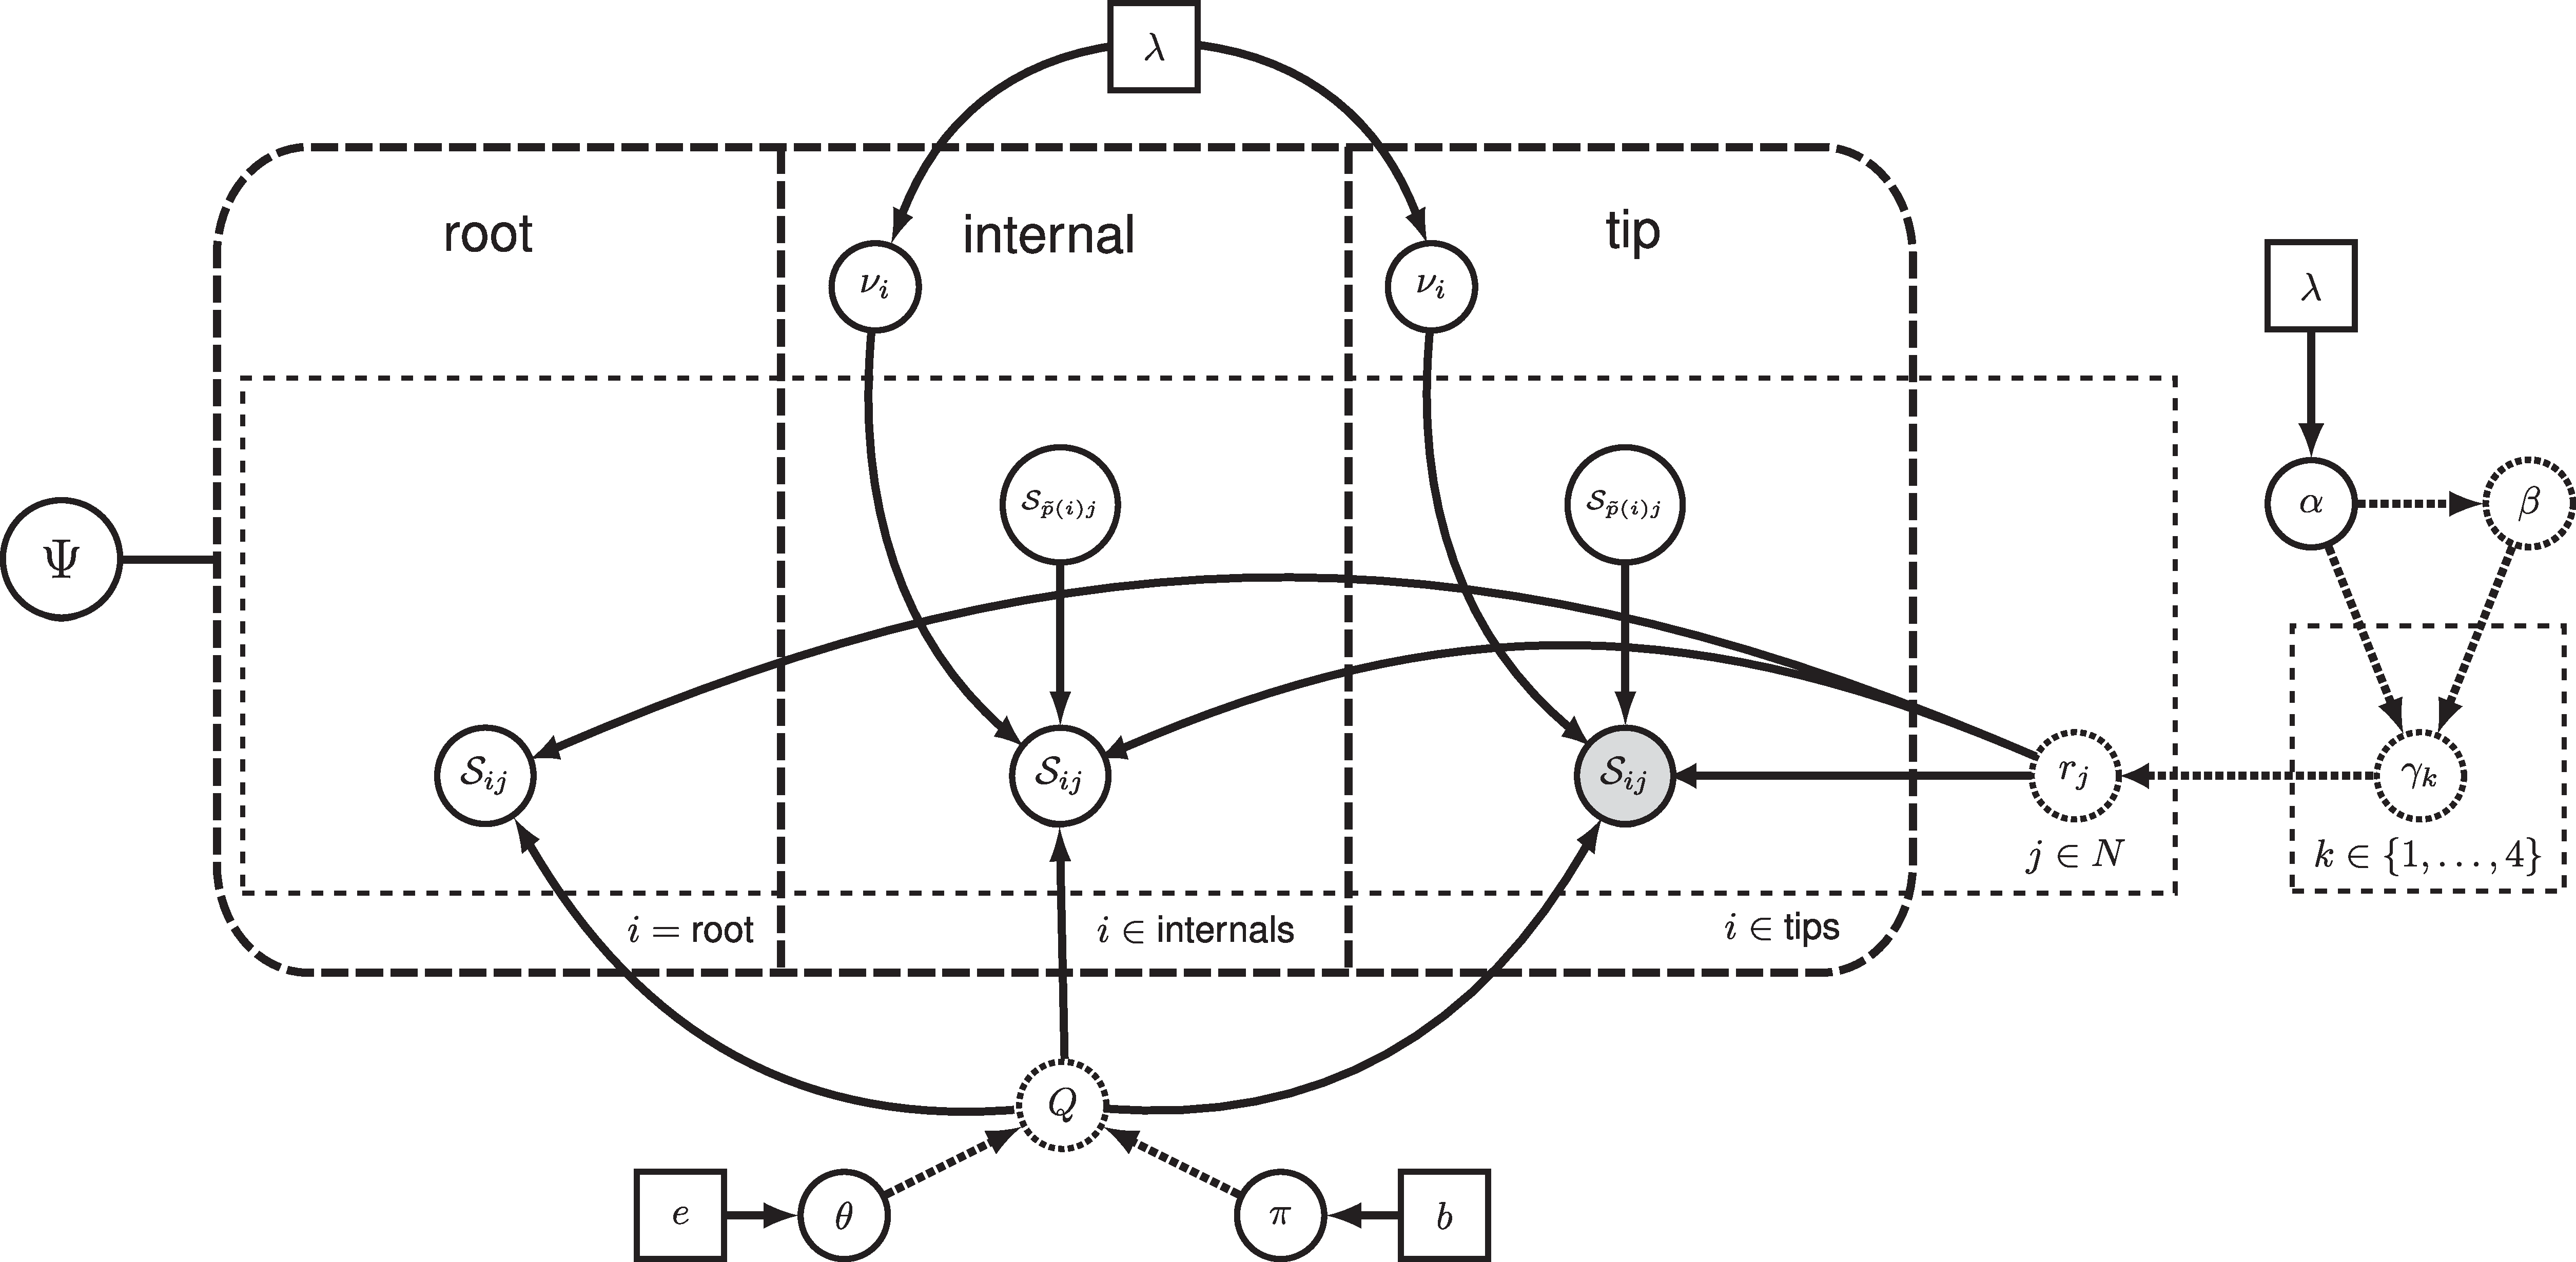
\includegraphics[width=\textwidth,angle=0]{\ResourcePath figures/gtrg_graphical_model_2.pdf}}
\caption{\small Graphical model representation of the General Time Reversible (GTR) + Gamma phylogenetic model.}
\label{fig:gtrg}
\end{figure}

\subsection{Setting up the Gamma Model in \RevBayes}

Create a constant node called \cl{shape\_prior} for the rate parameter of the exponential prior on the gamma-shape parameter (this is represented as the constant $\lambda$-rate parameter in Figure \ref{fig:gtrg}):
{\tt\begin{snugshade*}
\begin{lstlisting}
shape_prior <- 0.05                                                                             
\end{lstlisting}
\end{snugshade*}}
% I changed this from ``alpha_prior'' to match the description in the text

Then create a stochastic node called \cl{alpha} with an exponential prior (this represents the stochastic $\alpha$-shape parameter node $\alpha$ in Figure \ref{fig:gtrg}):
% The GTR+G graphical model figure was not previously included...I added a modified version below that 
% horizontally compressed the GTR part of the model; the modified version is called `gtrg_graphical_model_2.'
% I changed this from \cl{shape} in tis sentence to \cl{alpha} so that it matched the description in the code and the GTR + G graphical model description
{\tt\begin{snugshade*}
\begin{lstlisting}
alpha ~ dnExponential(shape_prior)
\end{lstlisting}
\end{snugshade*}}
% I changed this from ``alpha_prior'' to match the description in the txt

The way the ASRV model is implemented involves discretizing the mean-one gamma distribution into a set number of rate categories, $k$. 
Thus, we can analytically marginalize over the uncertainty in the rate at each site. 
The likelihood of each site is averaged over the $k$ rate categories, where the rate multiplier is the mean (or median) of each of the discrete $k$ categories. 
To specify this, we need a deterministic node that is a vector of rates calculated from the gamma distribution and the number of rate categories, $k$. 
The \cl{fnDiscretizeGamma()} function returns this deterministic node and takes three arguments: the shape and rate of the gamma distribution and the number of categories. 
Since we want to discretize a mean-one gamma distribution, we can pass in \cl{alpha} for both the shape and rate.
% I changed this from \cl{shape} in tis sentence to \cl{alpha} so that it matched the description in the code and the GTR + G graphical model description

Initialize the \cl{gamma\_rates} deterministic node vector using the  \cl{fnDiscretizeGamma()} function with \cl{4} bins:
{\tt \begin{snugshade*}
\begin{lstlisting}
gamma_rates := fnDiscretizeGamma( alpha, alpha, 4 )
\end{lstlisting}
\end{snugshade*}}

Note that here, by convention, we set $k = 4$.
The random variable that controls the rate variation is the stochastic node \cl{alpha}. 
% I changed this from \cl{shape} in tis sentence to \cl{alpha} so that it matched the description in the code and the GTR + G graphical model description
We will apply a simple scale move to this parameter.
{\tt \begin{snugshade*}
\begin{lstlisting}
moves[++mi] = mvScale(alpha, weight=2.0)
\end{lstlisting}
\end{snugshade*}}

Remember that you need to call the \cl{PhyloCTMC} constructor to include the new site-rate parameter:
% This sentence was incomplete previously; I think the revised version is correct.
{\tt \begin{snugshade*}
\begin{lstlisting}
seq ~ dnPhyloCTMC(tree=phylogeny, Q=Q, siteRates=gamma_rates , type="DNA")
\end{lstlisting}
\end{snugshade*}}


\subsection{Execise 4}

Modify the previous GTR analysis to specify the GTR+Gamma model. 
Run an MCMC simulation to estimate the posterior distribution.
\begin{itemize}
\item Is there an impact on the estimated phylogeny compared with the previous analyses? 
	Look at the MAP tree and the posterior probabilities of the clades.
\item What is the estimated tree length? 
	Is the estimate different to the previous analysis? What could cause this?
\item Complete the table of the phylogenetic relationship of Tarsiers.
\end{itemize}



\newpage
\section{Modeling Invariable Sites}
All of the substitution models described so far assume that the sequence data are potentially variable.
That is, we assume that the sequence data are random variables; specifically, we assume that they are realizations of the specified \cl{PhyloCTMC} distribution. 
However, some sites may not be free to vary---when the substitution rate of a site is zero, it is said to be \emph{invariable}.
Invariable sites are often confused with \emph{invariant} sites---when each species exhibits the same state, it is said to be invariant.
The concepts are related but distinct.
If a site is truly invariable, it will necessarily give rise to an invariant site pattern, as such sites will always have zero substitutions.
However, an invariant site pattern may be achieved via multiple substitutions that happen to end in the same state for every species.

Here we describe an extension to our phylogenetic model to accommodate invariable sites.
Under the invariable-sites model \citep[][]{Hasegawa1985}, each site is invariable with probability \cl{pinvar}, and variable with probability $1-pinvar$.

First, let's have a look at the data and see how many invariant sites we have:
{\tt \begin{snugshade*}
\begin{lstlisting}
data.getNumInvariantSites()
\end{lstlisting}
\end{snugshade*}}
There seem to be a substantial number of invariant sites.

Now let's specify the invariable-sites model in \RevBayes.
We need a prior probability for the probability of a site being invariable.
A Beta distribution is a common choice for parameters representing probabilities.
{\tt \begin{snugshade*}
\begin{lstlisting}
pinvar ~ dnBeta(1,1)
\end{lstlisting}
\end{snugshade*}}
The \cl{Beta(1,1)} distribution is a flat prior distribution that specifies equal probability for all values between 0 and 1.

Then, as usual, we add a move to change this stochastic variable; we'll used a simple sliding window move.
{\tt \begin{snugshade*}
\begin{lstlisting}
moves[mi++] = mvSlide(pinvar)
\end{lstlisting}
\end{snugshade*}}

\subsection{Exercise 5}

\begin{itemize}
\item Extend the GTR model to account for invariable sites and run an analysis.
\item What is the estimated probability of invariable sites and how does it relate to the ratio of invariant sites to the total number of sites?
\item Extend the GTR+$\Gamma$ model to account for invariable sites and run an analysis.
\item What is the estimated probability of invariable sites now?
\item Complete the table of the phylogenetic relationship of Tarsiers.
\end{itemize} 

\vspace{5cm}
Questions about this tutorial can be directed to: \\\vspace{-10mm}
\begin{itemize}
\item Tracy Heath (email: \href{mailto:tracyh@berkeley.edu}{tracyh@berkeley.edu}) \\\vspace{-8mm}
\item Michael Landis (email: \href{mailto:mlandis@berkeley.edu}{mlandis@berkeley.edu}) \\\vspace{-8mm} 
\item Sebastian H\"{o}hna (email: \href{mailto:sebastian.hoehna@gmail.com}{sebastian.hoehna@gmail.com}) \\\vspace{-8mm}
\item Brian R. Moore (email: \href{mailto:brianmoore@ucdavis.edu}{brianmoore@ucdavis.edu}) \\\vspace{-8mm}
\end{itemize}

\bibliographystyle{sysbio}
\bibliography{\ResourcePath refs}
